Der folgende Abschnitt stellt drei reale Fallbeispiele vor.
\subsection{Quirky}
Quirky ist ein Unternehmen gegr�ndet von Ben Kaufman, welches in New York City angesiedelt ist. Die Gesch�ftsidee besteht darin eine �ffentlich zug�ngliche Onlineplattform einzurichten und �ber diese jedem einzelnen die M�glichkeit zu geben Produktideen vorzustellen(fr�her gegen eine Geb�hr). Andere User k�nnen nunmehr die Produktideen bewerten und Kommentieren. Kommen bei einer Produktidee gen�gend positive R�ckmeldungen wird das Produkt gemeinsam mit der Community entwickelt. Hier ist schon zu erkennen, dass die Community einen wichtigen Bestandteil des Unternehmens darstellt. Abbildung \ref{quirkySystem} zeigt den Einfluss der Community noch einmal grafisch. Um eine m�glichst starke Community aufzubauen ben�tigt es nat�rlich Anreize um die einzelnen User an das Unternehmen zu binden. Quirky verfolgt hier ma"sgeblich den monet�ren Ansatz und bietet laut einem Werbeslogan auf ihrer Website schon f�r einen Klick eine finanzielle Verg�tung.
\begin{figure}[h!]
	\caption{�bersicht �ber den Crowdsourcing-Prozess bei Quirky\cite{TENREASONSQUIRKY}}
	\centering
		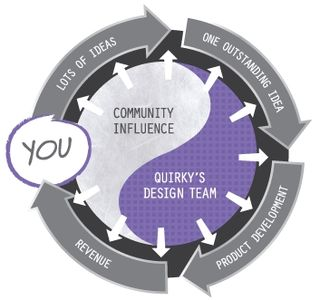
\includegraphics[scale=0.9]{figures/Quirky}
\label{quirkySystem}
\end{figure}

Hierbei ist anzumerken, dass Quirky ein hybrides Modell an Community-Beteiligung und eigener Entwicklung nutzt. Quirky k�mmert sich um die Koordination sowie um die schwierigeren Entwicklungsschritte, wie zum Beispiel die technische Entwicklung des Produkts.

Quirky vertraut bei diesem Gesch�ftsmodell haupts�chlich auf die sogenannten Lead-User, welche in den vorangegangen Kapiteln genauer beschrieben wurden. Eine neue Idee einzureichen ist relativ einfach m�glich �ber die angebotene Online-Plattform(\url{www.quirky.com}). Es wird ein Titel, eine sogenannte \glqq Elevator Pitch\grqq (kurze Beschreibung des Produkts), eine Einteilung in eine von insgesamt 8 Kategorien anschlie"send ist zu beantworten welches Problem die Idee l�st und wie das Problem gel�st werden kann.

Ein anderer wichtiger Teil bei der Produktentwicklung ist die Beeinflussung der urspr�nglichen Produktidee durch die anderen Community-Mitglieder. Hierf�r wurde von Quirky ein System entwickelt mit sogenannten Influence-Punkten, welche prozentuell vergeben werden. Diese Influence-Punkte geben an inwieweit ein User die Entwicklung eines Produktes beeinflusst hat. Entsprechend dieser Verteilung erfolgt die Aufteilung der Gewinne die mit dem Produkt gemacht werden. Zu beachten ist jedoch, dass man nur Aussicht auf eine finanzielle Verg�tung besitzt, falls das Produkt auch wirklich auf den Markt gebracht wird. Insgesamt sch�ttet Quirky 10\% des Gewinns welches mit dem Produkt gemacht wird an seine Community aus. In Abbildung \ref{quirkyInfluence} wird noch einmal verdeutlicht wie die Influence-Punkte auf die Community aufgeteilt werden.

\begin{figure}[h!]
	\caption{Aufteilung der Influence-Punkte auf die einzelnen Entwicklungsstufen\cite{QUIRKYCOMINF}}
	\centering
		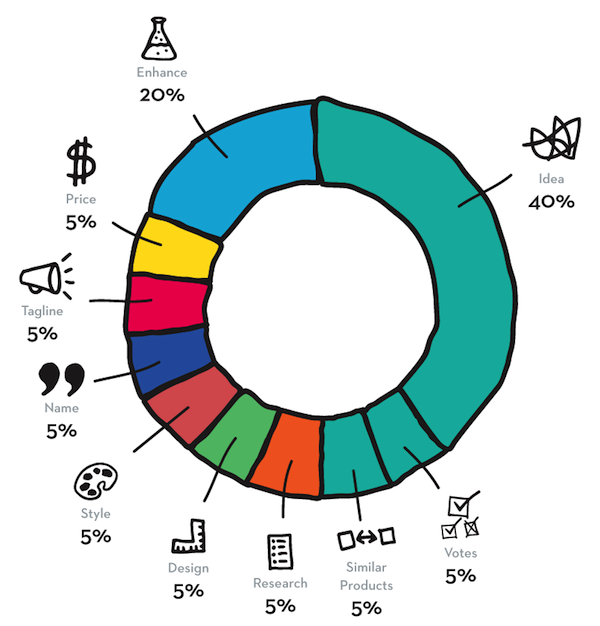
\includegraphics[scale=0.8]{figures/influence-chart1}
	\label{quirkyInfluence}
\end{figure}

Ein Nachteil der finanziellen Verg�tung in der Form wie sie Quirky anwendet, bei der man bei jeder Interaktion mit der Community Geld verdient ist, dass es zwar viele Interaktionen der Community gibt, jedoch die Qualit�t der Kommentare, Votings(man Voted f�r das bereits beste Produkt) fraglich ist. Quirky scheint dieses Problem jedoch nicht zu haben.

Ein weiteres Problem stellt die Abtretung der Rechte des Lead-Users dar, falls die Produktidee von Quirky angenommen wird. Es besteht zwar ein Anspruch auf eine entsprechende Verg�tung durch Quirky, jedoch wenn Patente angemeldet werden ist es fraglich wer als Erfinder eingetragen wird. Oftmals werden Produktideen von mehr als 800 Personen beeinflusst. Hier stellt sich die Frage ob nicht Plattformen wie Kickstarter und co. besser geeignet sind gute Ideen umzusetzen und zu finanzieren, da hier die Rechte bei den Erfindern bleiben.
\cite{LOSINGRIGHTS}

Quirky hat mit Stand Dezember 2013 eine globale Community von 600000 Mitglieder, die Produkte entwerfen und beeinflussen.\cite{REPORTQUIRKY2345}


\subsection{InnoCentive}
TODO

\subsection{Crowdspirit}
TODO fehlgeschlagene Crowdsourcing plattform